\chapter{Attacco all'autenticazione delle reti 5G}
In questa sezione verranno trattate le vulnerabilità riguardo un attacco di tipo \textit{Denial of Service} all'autenticazione delle reti 5G.
Questa generazione ha risolto alcune delle probematiche legate all'autenticazione, come per esempio a differenza del 4G (LTE) l'identificatore 
dello UE viene criptato con la chiave pubblica prima di essere inviato al \textit{Core network}, evitando così di poter essere intercettato e rubato\cite{5g-vs-4g}.
Però, con il grande aumento di dispositivi connessi che questa tecnologia vuole incentivare, per esempio nel mondo dell' IOT, gli attacchi DOS saranno senz'altro più 
semplici da realizzare.\\
I SDN e NFV, componenti fondamentali per garantire le eccezionali prestazioni del 5G, potrebbero essere un efficace strumento di monitoraggio per identificare possibili 
attacchi come spiegato in \cite{dos-detection-with-sdn}.\\
Allo stesso tempo però, la centralizzazione del controllo del \textit{network} con un SDN e NFV crea le condizioni ottimali per effettuare un attacco DOS con successo\cite{5g-dos}.\\
Questa tipologia di attacchi che ha lo scopo di creare unainterruzione del servizio hanno una pericolosià maggiore in questa generazione. Infatti, il mondo dell'IOT e le smart cities comprendono 
dispositivi sensibili come per esempio il mondo della telemedicina.

\section{IMSI \textit{catching}}
Come anticipato, l'avanzamento più importante in termini di sicurezza che questa nuova generazione ha apportato è sicuramente la trasmissione dell'identificativo del MS o UE in forma 
criptata. Questa innovazione ha reso molto più difficile la pratica dell'IMSI \textit{catching} trattata nella sezione (?) fondamentale per Successivamente effettuare un attacco DOS.\\
Realisticamente però bisogna sottolineare che questa pratica non risulta completamente debellata. Infatti, tutte le nuove reti 5G, come è stato anche per le generazioni precedenti, devono 
essere retro compatibili, e quindi per un non determinato lasso di tempo devono essere supportate le procedure degli \textit{standard} precedenti che, come spiegato nel capitolo precedente, soffrono 
di questa vulnerabilità.\\
In \cite{suci-catch} viene illustrato un metodo per effettuare un attacco MITM nelle reti 5G in modo da ottenere l'IMSI criptato dell'utente: il SUCI. Questo metodo però non sarebbe applicabile per effettuare 
una raccolta di identificativi per poi effettuare un attacco DOS poichè il SUCI viene rigenerato dopo ogni utilizzo.
\begin{figure}[ht]
    \centering
    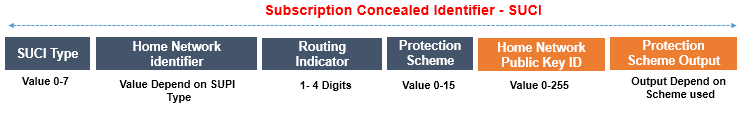
\includegraphics[width=0.8\textwidth]{images/5g-suci.png}
    \caption{Composizione del SUCI nel 5G}
\end{figure}

\clearpage

\section{Replicazione dell'attacco SIM-less}
Alla base degli attacchi trattati nella sezione 6.3 vi è la costruzione di un \textit{database} di IMSI. Questo database può essere agevolmente costruito nelle generazioni precedenti al 5G 
tramite le tecniche di IMSI \textit{catching} trattate in 6.2. Nel 5G risulta molto più difficile creare un archivio di IMSI poichè questi viaggiano in forma criptata nella rete ovvero il SUCI.\\
Tuttavia, se si riuscisse a ottenere comunque un \textit{database} di IMSI rubati si potrebbe ottenere un attacco dello stesso tipo di \cite{gsm-dos-simless} e \cite{umts-dos} con prestazioni migliori 
perchè il nuovo protocollo 5G NR\cite{5g-nr} per l'\textit{air interface} è stato progettato per supportare il \textit{Massive Machine Type Communications} ovvero l'IOT massivo che richiede latenze molto basse e capacità molto alte.
Per questo, sicuramente la capacità dei canali di comunicazione durante la procedura di autenticazione avrebero un valore di TPS molto alto, sufficiente a causare un notevole degradamento delle prestazioni.

\section{Nuove vulnerabilità}
L'implementazione del SUCI e SUPI ha risolto, o quantomeno reso molto più complicata la pratica dell'IMSI \textit{catching}. Allo stesso tempo però ha incrementato il dispendio di risorse durante l'autenticazione
di un dispositivo. Come è chiaramente visibile nell'immagine sottostante, prima della generazione dei vettori di autenticazione vengono innestate delle procedure per decriptare il SUCI che avvengono con un algoritmo detto 
\textit{Elliptic Curve Integrated Encryption Scheme} (ECIES). 
Questa procedura aumenta inevitabilmente la creazione di possibili DOS all'autentcazione. 
In \cite{5g-lightweight} è descritto un protocollo che permetterebbe di controllare fin dal primo momento se il MS ha un SUCI valido senza incorrere nella decriptazione.
